\documentclass[10pt]{beamer}\usepackage[]{graphicx}\usepackage[]{xcolor}
% maxwidth is the original width if it is less than linewidth
% otherwise use linewidth (to make sure the graphics do not exceed the margin)
\makeatletter
\def\maxwidth{ %
  \ifdim\Gin@nat@width>\linewidth
    \linewidth
  \else
    \Gin@nat@width
  \fi
}
\makeatother

\definecolor{fgcolor}{rgb}{0.345, 0.345, 0.345}
\newcommand{\hlnum}[1]{\textcolor[rgb]{0.686,0.059,0.569}{#1}}%
\newcommand{\hlstr}[1]{\textcolor[rgb]{0.192,0.494,0.8}{#1}}%
\newcommand{\hlcom}[1]{\textcolor[rgb]{0.678,0.584,0.686}{\textit{#1}}}%
\newcommand{\hlopt}[1]{\textcolor[rgb]{0,0,0}{#1}}%
\newcommand{\hlstd}[1]{\textcolor[rgb]{0.345,0.345,0.345}{#1}}%
\newcommand{\hlkwa}[1]{\textcolor[rgb]{0.161,0.373,0.58}{\textbf{#1}}}%
\newcommand{\hlkwb}[1]{\textcolor[rgb]{0.69,0.353,0.396}{#1}}%
\newcommand{\hlkwc}[1]{\textcolor[rgb]{0.333,0.667,0.333}{#1}}%
\newcommand{\hlkwd}[1]{\textcolor[rgb]{0.737,0.353,0.396}{\textbf{#1}}}%
\let\hlipl\hlkwb

\usepackage{framed}
\makeatletter
\newenvironment{kframe}{%
 \def\at@end@of@kframe{}%
 \ifinner\ifhmode%
  \def\at@end@of@kframe{\end{minipage}}%
  \begin{minipage}{\columnwidth}%
 \fi\fi%
 \def\FrameCommand##1{\hskip\@totalleftmargin \hskip-\fboxsep
 \colorbox{shadecolor}{##1}\hskip-\fboxsep
     % There is no \\@totalrightmargin, so:
     \hskip-\linewidth \hskip-\@totalleftmargin \hskip\columnwidth}%
 \MakeFramed {\advance\hsize-\width
   \@totalleftmargin\z@ \linewidth\hsize
   \@setminipage}}%
 {\par\unskip\endMakeFramed%
 \at@end@of@kframe}
\makeatother

\definecolor{shadecolor}{rgb}{.97, .97, .97}
\definecolor{messagecolor}{rgb}{0, 0, 0}
\definecolor{warningcolor}{rgb}{1, 0, 1}
\definecolor{errorcolor}{rgb}{1, 0, 0}
\newenvironment{knitrout}{}{} % an empty environment to be redefined in TeX

\usepackage{alltt}

%\usetheme{metropolis}
\usetheme[progressbar=head]{metropolis}
\defaultfontfeatures{ Scale = MatchUppercase }
\defaultfontfeatures[\rmfamily]{ Scale = 1}
\usepackage{unicode-math}

\usepackage{fontspec}
%\setmainfont[Scale = 0.95]{Lucida Bright OT}
%\setsansfont[Scale = 0.95]{Lucida Sans OT}
%\setmonofont[Scale = 0.80]{Lucida Console DK}

%\newfontfamily\meteoconsfont{Meteocons}
%\newcommand\meteocons[1]{{\meteoconsfont\symbol{#1}}}
%\newcommand\meteosun{\meteocons{"0042}}
%\newcommand\meteosuncloud{\meteocons{"0048}}
%\newcommand\meteorain{\meteocons{"0052}}
%\newcommand\meteosolidsun{\meteocons{"0031}}

\newfontfamily\lineabasicfont{linea-basic-10}
\newcommand\basicicons[1]{{\lineabasicfont\symbol{#1}}}
\newcommand\timeforwards{\basicicons{"0079}}
\newcommand\timebackwards{\basicicons{"0064}}

\newfontfamily\lineaweatherfont{linea-weather-10}
\newcommand\weathericons[1]{{\lineaweatherfont\symbol{#1}}}
\newcommand\meteosun{\weathericons{"E038}}
\newcommand\meteosuncloud{\weathericons{"E042}}
\newcommand\meteorain{\weathericons{"E033}}
\newcommand\meteowind{\weathericons{"E054}}

\newfontfamily\uleaffont{Mini Pics Uprooted Leaf}
\newcommand\uleafmpics[1]{{\uleaffont\symbol{#1}}}
\newcommand\lowplants{\uleafmpics{"00CE}}
\newcommand\mediumplant{\uleafmpics{"006A}}
\newcommand\bush{\uleafmpics{"0039}}
\newcommand\smallplant{\uleafmpics{"0030}}

\newfontfamily\KRfarmfont{KR Back On The Farm}
\newcommand\KRfarm[1]{{\KRfarmfont\symbol{#1}}}
\newcommand\farmplant{\KRfarm{"0049}}

\usepackage{framed}

\usepackage{tikz}
\usetikzlibrary{positioning,fit,arrows}

\tikzset{
 a/.style
  = {node distance=4em, text width=2.7em, minimum height=4em},
 b/.style
  = {rectangle, draw, fill=gray!10, node distance=4em, text width=6em,
     text centered, rounded corners, minimum height=4em, thick},
 c/.style
  = {circle, draw, dashed, fill=orange!10, inner sep = 0pt, node distance=5em, thick},
 d/.style
  = {rectangle, draw, dashed, fill=red!10, node distance=4em, text width=6em,
     text centered, rounded corners, minimum height=4em, thick},
 l/.style
  = {draw, -latex, thick},
 lr/.style
  = {draw, latex-latex, thick, red},
 lb/.style
  = {draw, -latex, thick, blue},
  lo/.style
  = {draw, -latex, thick, orange},
  lg/.style
  = {draw, -latex, thick, green},
  mylabel/.style
  ={text width=6.5em, text centered}
}

\usepackage{abbrev}

%\usepackage[style=authoryear-comp,firstinits,sortcites,maxcitenames=2,%
%    mincitenames=1,maxbibnames=10,minbibnames=10,uniquename=mininit,%
%    uniquelist=minyear,sortfirstinits=true]{biblatex}
%\usepackage[backend=biber,style=alphabetic]{biblatex}
\usepackage[style=authoryear-comp,firstinits,sortcites,maxcitenames=2,%
    mincitenames=1,maxbibnames=10,minbibnames=10,uniquename=mininit,%
    uniquelist=minyear,sortfirstinits=true]{biblatex}
\addbibresource{info4plants.bib}
%\renewcommand{\bibfont}{\small}
\IfFileExists{upquote.sty}{\usepackage{upquote}}{}
\begin{document}





\pgfdeclareimage[height=10ex]{SenPEP_large}{figures/senpep_logo}
\pgfdeclareimage[width=0.19\textwidth]{SenPEP}{figures/senpep_logo}
\pgfdeclareimage[width=0.19\textwidth]{HYflame}{figures/HY_biot_text}
\pgfdeclareimage[width=0.15\textwidth]{ViPS}{figures/senpep_logo}
\pgfdeclareimage[width=0.12\textwidth]{SMS}{figures/SMS}
\pgfdeclareimage[width=0.11\textwidth]{ESP}{figures/ESP}
\pgfdeclareimage[width=0.15\textwidth]{ViPS}{figures/vips-logo}
\pgfdeclareimage[width=0.15\textwidth]{AKA}{figures/aka_logo}

\title{The importance of context\\in plant biology}
\subtitle{A possible framework for its analysis}
\author{Pedro J. Aphalo}
\date{Adelaide, 27 November 2018}
\institute[Univ.\ of Helsinki]{Organismal and Evolutionary Biology Research Programme\\[1ex] and\\[1ex] Viikki Plant Science Center, University of Helsinki\\[1ex] \href{http://blogs.helsinki.fi/senpep-blog/}{\pgfuseimage{SenPEP_large}} }


	\begin{frame}
		\maketitle
	\end{frame}

	\begin{frame}[c]
		\begin{center}
			\begin{small}
				\copyright 2016--2018 by Pedro J. Aphalo\\
				Organismal and Evolutionary Biology Research Programme, University of Helsinki, Finland.\\
				\textcolor{blue}{\url{http://blogs.helsinki.fi/senpep-blog/}}\\[2ex]
			\end{small}

			\begin{footnotesize}
				`The importance of context in plant biology' slides from a presentation by Pedro J. Aphalo are licensed under a Creative Commons Attribution-ShareAlike 4.0 International License.\\[2ex]

			\end{footnotesize}

			
\includegraphics[width=6em]{figures/by-sa}
		\end{center}
	\end{frame}

	\begin{frame}
		\frametitle{Outline}
		\tableofcontents
	\end{frame}

\section{Background}

\begin{frame}%[<+->]
  \frametitle{An evolutionary viewpoint}
  \begin{itemize}
    \item The focus of my presentation will be the sensory abilities of plants from an evolutionary and fitness perspective.
    \item Fitness represents an \emph{ultimate cause} (a \emph{why} question).
    \item The physiological and/or molecular mechanisms are \emph{proximate causes} (\emph{how} questions).
    \item In animal ecology sensory ecology is an important discipline.
    \item In the case of plants this approach has been rarely used\ldots
    \item \ldots based on the assumption that sensory capabilities and specially information processing are very limited in plants.
    \item Now we know that this assumption does not hold.
  \end{itemize}
\end{frame}

\begin{frame}%[<+->]
  \frametitle{Vocabulary: information as an abstraction}
  \begin{itemize}
    \item (A technological example is radio broadcasting vs.\ internet-``radio'' vs.\ radio communication.)
    \item First a signal (or cue) needs to be sensed or perceived.
    \item A signal may carry information or not, if it does not carry information we call it ``noise''.
    \item To extract information a signal must be decoded.
    \item Memory is the storage of information.
    \item Processing is the combination of different bits of information.
    \item Communication is the exchange of information (there is an emitter and a receiver, can be one-way or two way).
  \end{itemize}
\end{frame}

\begin{frame}%[<+->]
  \frametitle{Forecasting: its relation to fitness}
  \begin{itemize}
\item Our everyday life depends on forecasting all sorts of events every minute.
    \item Sometimes we do this consciously, but most of the time we are not aware of what our brain is doing.
    \item We use forecasts at very different time scales and to many different ends (e.g.\ estimating the weight of a cup when lifting it).
    \item I will use the abstraction of \emph{information}, and for a moment I will ask you to forget about how its processing is implemented\ldots
    \item \ldots and consider the idea that every organism must have evolved the capacity to ``forecast'' future events important for fitness.
    \item How information is processed, ``the machinery used'', does not need to be the same as long the information is acquired, transmitted, stored and combined successfully.
    \item The discussion of the role of ``future perception'' in fitness of plants is current \autocite{Novoplansky2016a}.
  \end{itemize}
\end{frame}

\begin{frame}%[<+->]
  \frametitle{Can plants forecast? Preemptive acclimation}
   \begin{itemize}
    \item Several plant responses can be only explained from the evolutive/fitness
    point of view as being a `preparation' to tolerate or escape future stress events or
    to take advantage of future favourable conditions.
    \begin{itemize}
    \item Example 1: Phenology.
    \item Example 2: Preemptive shade avoidance as a response to reflected far-red light from neighbouring
    plants.
    \item Example 3: Eavesdropping-on/communicating-with neighbours to preemptively acclimate/prepare
    for drought, herbivore attacks, even to synchronize flowering among individuals.
    \item Example 4: Possibly (a hypothesis) preemptive acclimation to future soil
    drying in response to high ultraviolet-B irradiance.
 \end{itemize}
  \end{itemize}
\end{frame}

\section{Why sensory ecology?}

%\begin{frame}[<+->]
%\frametitle{Sensory ecology approach}
%\begin{enumerate}
%  \item Focus on the acquisition and use of information by organisms
%  \item Well developed discipline for animals
%  \item Less developed for plants
%  \item Why?
%  \item \ldots plants' behaviour is not easy for humans to observe (slow\ldots)
%  \item \ldots intellectually we find the idea of brainless organisms \emph{solving problems} and \emph{assessing risks} alien
%  \item In abstract terms of flow, exchange, storage and use of information the concept of \emph{organisms as problem solvers} makes a lot of sense for any organism\ldots
%\end{enumerate}
%\end{frame}

\begin{frame}%[<+->]
\frametitle{My view on the role of information}
\begin{enumerate}
  \item Information sources are crucial to the performance and survival of organims\ldots
  \item \ldots $\Rightarrow$ cross-correlations among variables in their environment and their lags, and autocorrelations, are key sources of information
  \item \ldots $\Rightarrow$ we need to pay attention to `joint statistical properties of environmental variables'\ldots
  \item We need to pay more attention to the sources of information\ldots
  \item \ldots and how sensory mechanisms have been ``tuned'' by evolution to filter information from noise.
\end{enumerate}
\end{frame}

\begin{frame}
  \frametitle{Correlations in the environment}
  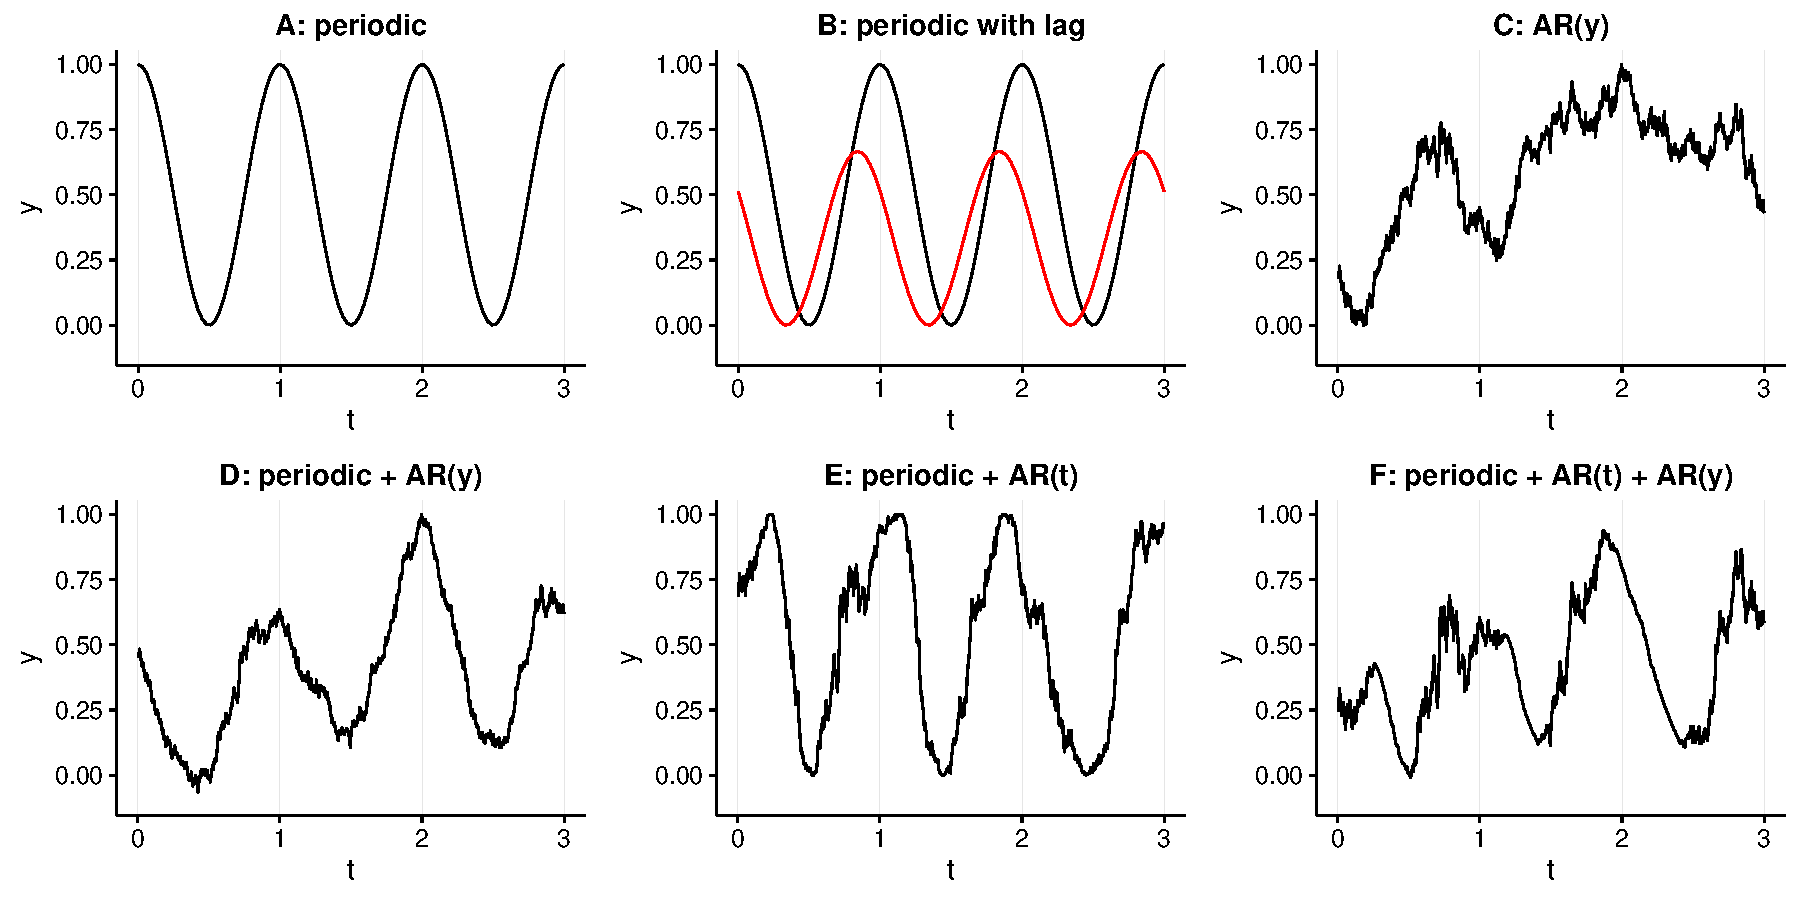
\includegraphics[width=\linewidth]{figures/cor_examples2.pdf}
\end{frame}

\begin{frame}%[<+->]
\frametitle{Forecasting}
\begin{enumerate}
  \item Lagged cross-correlations and autocorrelations make it possible the modelling and short-term forecasting of non-deterministic variation.
  \item Organisms can generate ``correlated variables'' through the emission of signals that propagate faster than the event they have perceived.
  \item e.g.\ emission of volatile organic compounds in response to insect herbivory.
  \item e.g.\ release of ABA to the shared soil volume with drought or salinity.
  \item e.g.\ unknown signal in the soil inducing synchronization of flowering.
  \item \textbf{Constraint:} to persist during evolution signals must benefit the emitter!
\end{enumerate}
\end{frame}

\section{A possible framework}

\begin{frame}{Proposed theoretical framework (I)}

\begin{itemize}
\item<1-11>[]Conceptual framework\vspace{1ex}\pause

\centering
\resizebox{\linewidth}{!}{%
\tiny
  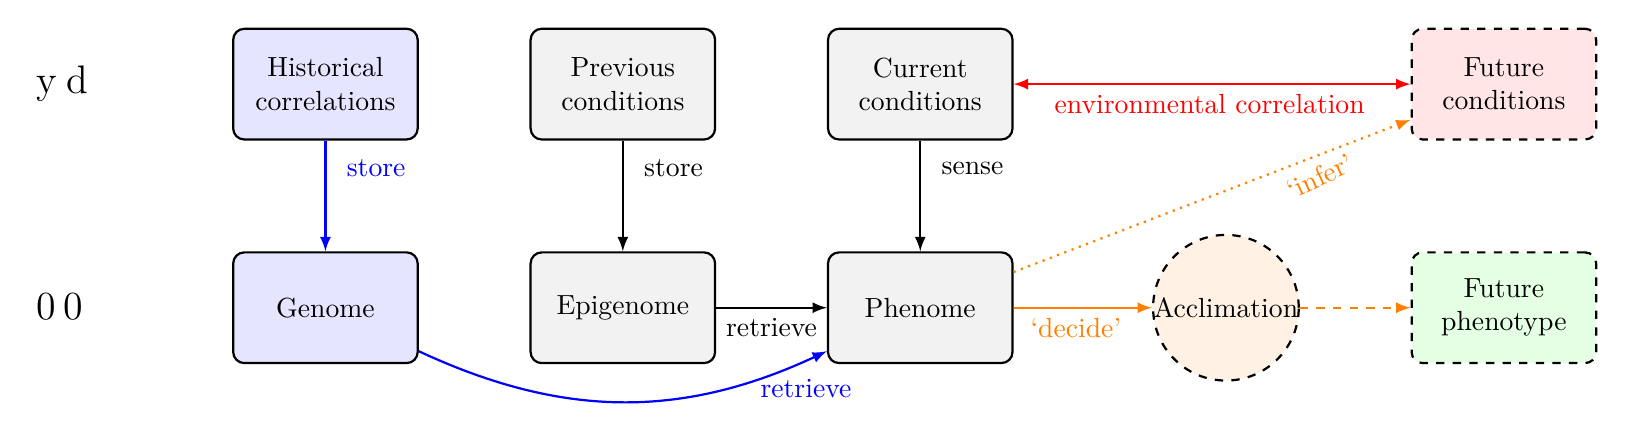
\begin{tikzpicture}[auto]
    \node [a] (environment) {\Large\timeforwards~\timebackwards};
    \node [b, right = of environment, fill=blue!10] (history) {Historical correlations};
    \node [b, right = of history] (stress) {Previous conditions};
    \node [b, right = of stress] (data) {Current conditions};\pause
    \node [b, below = of stress] (memory) {Epigenome};
    \node [b, right = of memory] (info) {Phenome};
    \node [b, below = of history, fill=blue!10] (genome) {Genome};
    \node [a, below = of environment] (plant) {\Large\smallplant\,\smallplant};\pause
    \node [c, right = of info, fill=orange!10] (acclimation) {Acclimation};
    \node [d, right = of acclimation, fill=green!10] (ready) {Future phenotype};
    \node [d, above = of ready] (stress2) {Future conditions};\pause

    \path [l] (stress) -- (memory) node[near start,right]{\hspace{0.4em}store};
    \path [lb] (history) -- (genome) node[near start, right]{\hspace{0.4em}store};\pause
    \path [l] (data) -- (info) node[near start,right]{\hspace{0.4em}sense};
    \path [l] (memory) -- (info) node[near start,below]{\hspace{2em}retrieve};
    \path [lb] (genome) edge [bend right=25]  node[near end, right]{\hspace{1em}retrieve} (info);\pause
    \path [lr] (stress2) -- (data) node[near end,below]{\hspace{7em}environmental correlation};\pause
    \path [lo, dotted] (info) -- (stress2) node[near end,below,rotate=25]{`infer'};\pause
    \path [lo] (info) -- (acclimation) node[near start,below]{\hspace{2em}`decide'};\pause
    \path [lo, dashed] (acclimation) -- (ready);

\end{tikzpicture}%
}%


\item<11>[]Example: Frost hardening\vspace{1ex}\pause

\centering
\resizebox{\linewidth}{!}{%
\tiny
  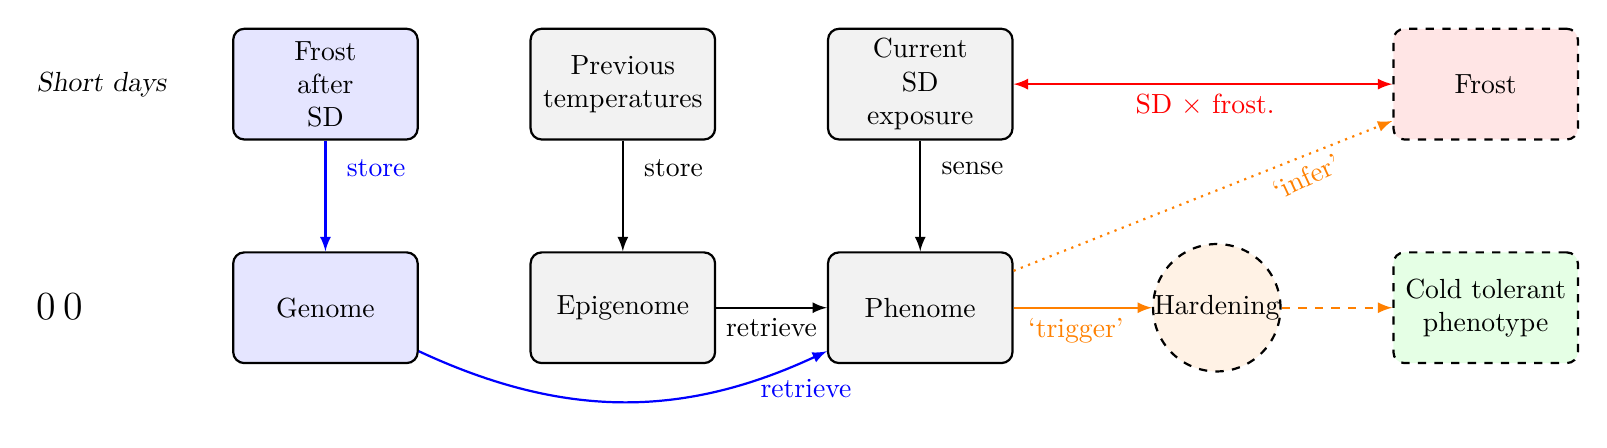
\begin{tikzpicture}[auto]
    \node [a] (environment) {\textsl{Short~days}};
    \node [b, right = of environment, fill=blue!10] (history) {Frost\\after\\SD};
    \node [b, right = of history] (stress) {Previous temperatures};
    \node [b, right = of stress] (data) {Current\\SD\\exposure};
    \node [b, below = of stress] (memory) {Epigenome};
    \node [b, right = of memory] (info) {Phenome};
    \node [b, below = of history, fill=blue!10] (genome) {Genome};
    \node [a, below = of environment] (plant) {\Large\smallplant\,\smallplant};
    \node [c, right = of info, fill=orange!10] (acclimation) {Hardening};
    \node [d, right = of acclimation, fill=green!10] (ready) {Cold tolerant phenotype};
    \node [d, above = of ready] (stress2) {Frost};

    \path [l] (stress) -- (memory) node[near start,right]{\hspace{0.4em}store};
    \path [lb] (history) -- (genome) node[near start, right]{\hspace{0.4em}store};
    \path [l] (data) -- (info) node[near start,right]{\hspace{0.4em}sense};
    \path [l] (memory) -- (info) node[near start,below]{\hspace{2em}retrieve};
    \path [lb] (genome) edge [bend right=25]  node[near end, right]{\hspace{1em}retrieve} (info);
    \path [lr] (stress2) -- (data) node[near end,below]{\hspace{7em}SD $\times$ frost.};
    \path [lo, dotted] (info) -- (stress2) node[near end,below,rotate=25]{`infer'};
    \path [lo] (info) -- (acclimation) node[near start,below]{\hspace{2em}`trigger'};
    \path [lo, dashed] (acclimation) -- (ready);

\end{tikzpicture}%
}%

\end{itemize}
%%\vspace{-6ex}
%\caption{\footnotesize\sffamily Information use in preemptive acclimation to drought by perception of UV-B radiation. Arrows represent flows of information: \textcolor{blue}{\textbf{blue}} = retrieved from genome (stored during earlier generations), \textbf{black} = acquired and/or `memorized' during an individual's lifetime, \textcolor{red}{\textbf{red}} = lagged correlation between UV-B radiation and drought (e.g.\ low soil water content and high evaporative demand), \textcolor{orange}{\textbf{orange}} = represents the outcome of `data processing'. The outcome is a `decision' on how to adjust function, morphology and development to achieve drought tolerance based on an `implicit forecast of impending drought'. Time runs from left to right, with dashed boxes representing the future. `Conditions' refer to both external environment and plant's internal status.}\label{fig:drought:info}
\end{frame}

\begin{frame}{Proposed theoretical framework (II)}

\begin{itemize}
\item<1-2>[]Conceptual framework\vspace{1ex}

\centering
\resizebox{\linewidth}{!}{%
\tiny
  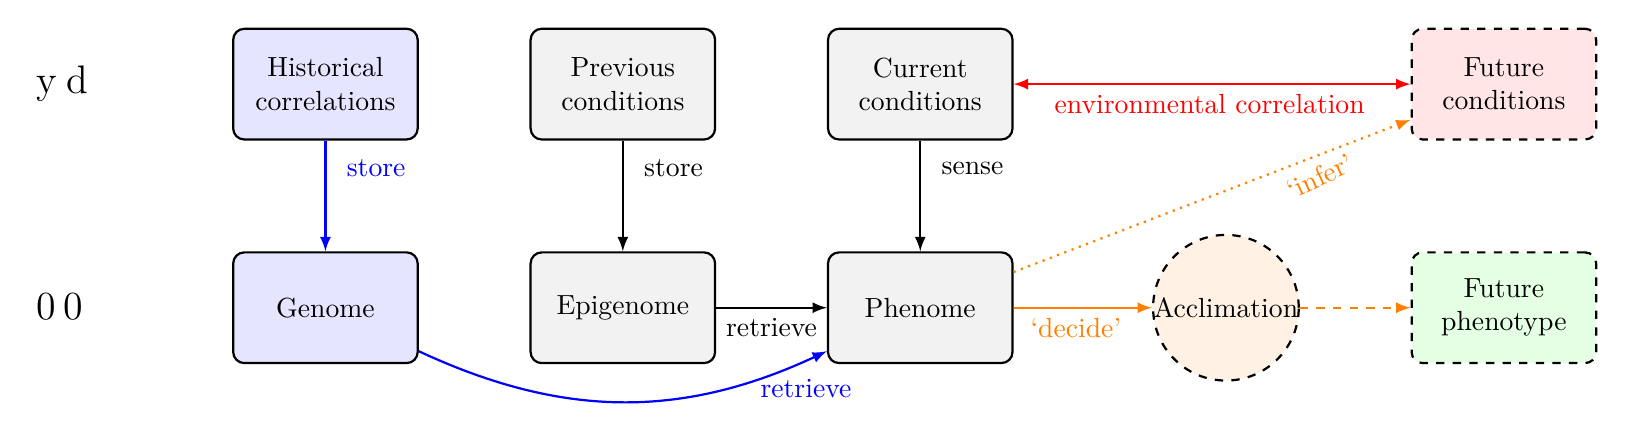
\begin{tikzpicture}[auto]
    \node [a] (environment) {\Large\timeforwards~\timebackwards};
    \node [b, right = of environment, fill=blue!10] (history) {Historical correlations};
    \node [b, right = of history] (stress) {Previous conditions};
    \node [b, right = of stress] (data) {Current conditions};
    \node [b, below = of stress] (memory) {Epigenome};
    \node [b, right = of memory] (info) {Phenome};
    \node [b, below = of history, fill=blue!10] (genome) {Genome};
    \node [a, below = of environment] (plant) {\Large\smallplant\,\smallplant};
    \node [c, right = of info, fill=orange!10] (acclimation) {Acclimation};
    \node [d, right = of acclimation, fill=green!10] (ready) {Future phenotype};
    \node [d, above = of ready] (stress2) {Future conditions};

    \path [l] (stress) -- (memory) node[near start,right]{\hspace{0.4em}store};
    \path [lb] (history) -- (genome) node[near start, right]{\hspace{0.4em}store};
    \path [l] (data) -- (info) node[near start,right]{\hspace{0.4em}sense};
    \path [l] (memory) -- (info) node[near start,below]{\hspace{2em}retrieve};
    \path [lb] (genome) edge [bend right=25]  node[near end, right]{\hspace{1em}retrieve} (info);
    \path [lr] (stress2) -- (data) node[near end,below]{\hspace{7em}environmental correlation};
    \path [lo, dotted] (info) -- (stress2) node[near end,below,rotate=25]{`infer'};
    \path [lo] (info) -- (acclimation) node[near start,below]{\hspace{2em}`decide'};
    \path [lo, dashed] (acclimation) -- (ready);

\end{tikzpicture}%
}%

\item<2>[]UVB example\vspace{1ex}

\centering
\resizebox{\linewidth}{!}{%
\tiny
  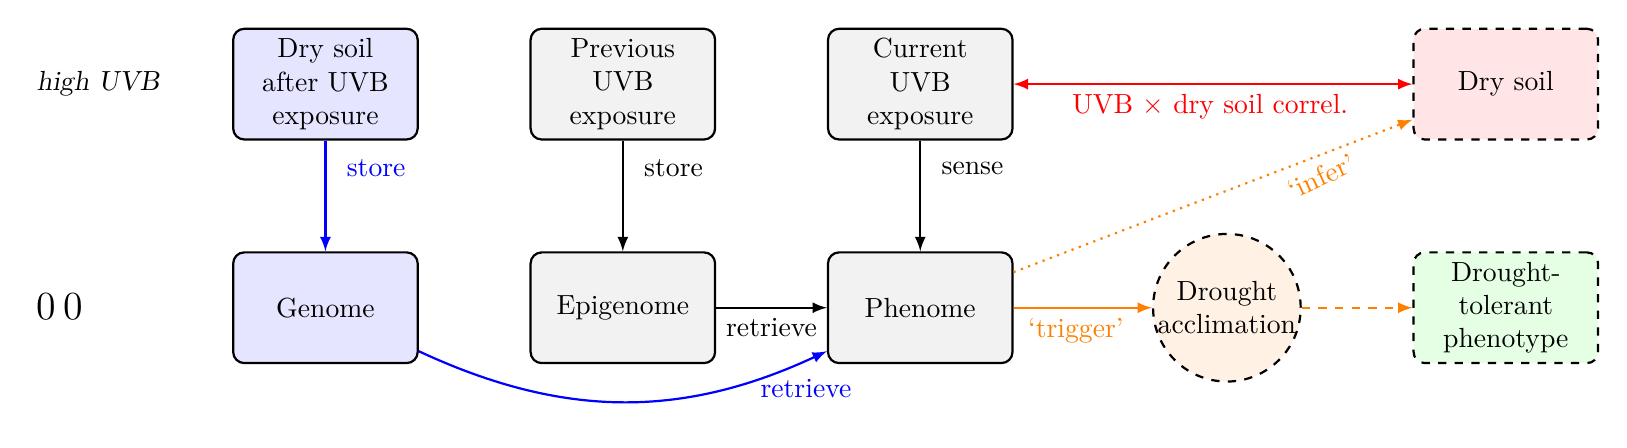
\begin{tikzpicture}[auto]
    \node [a] (environment) {\textsl{high~UVB}};
    \node [b, right = of environment, fill=blue!10] (history) {Dry soil\\ after UVB\\ exposure};
    \node [b, right = of history] (stress) {Previous\\ UVB\\ exposure};
    \node [b, right = of stress] (data) {Current\\ UVB\\ exposure};
    \node [b, below = of stress] (memory) {Epigenome};
    \node [b, right = of memory] (info) {Phenome};
    \node [b, below = of history, fill=blue!10] (genome) {Genome};
    \node [a, below = of environment] (plant) {\Large\smallplant\,\smallplant};
    \node [c, right = of info, fill=orange!10] (acclimation) {\parbox{5em}{\centering Drought\\ acclimation}};
    \node [d, right = of acclimation, fill=green!10] (ready) {Drought-tolerant phenotype};
    \node [d, above = of ready] (stress2) {Dry soil};

    \path [l] (stress) -- (memory) node[near start,right]{\hspace{0.4em}store};
    \path [lb] (history) -- (genome) node[near start, right]{\hspace{0.4em}store};
    \path [l] (data) -- (info) node[near start,right]{\hspace{0.4em}sense};
    \path [l] (memory) -- (info) node[near start,below]{\hspace{2em}retrieve};
    \path [lb] (genome) edge [bend right=25]  node[near end, right]{\hspace{1em}retrieve} (info);
    \path [lr] (stress2) -- (data) node[near end,below]{\hspace{7em}UVB $\times$ dry soil correl.};
    \path [lo, dotted] (info) -- (stress2) node[near end,below,rotate=25]{`infer'};
    \path [lo] (info) -- (acclimation) node[near start,below]{\hspace{2em}`trigger'};
    \path [lo, dashed] (acclimation) -- (ready);

\end{tikzpicture}%
}%


%\centering
%\tiny
%  \begin{tikzpicture}[auto]
%    \node [a, rotate=90] (environment) {\textsl{high~UVB}};
%    \node [b, right = of environment, fill=blue!10] (history) {dry soil\\ after UVB\\ exposure};
%    \node [b, below = of history, fill=blue!10] (genome) {Genome};
%    \node [a, rotate=90, left = of genome] (plant) {\textsl{Plant}};
%    \node [b, right = of history] (stress) {Recent\\ UVB\\ exposure};
%    \node [b, right = of stress] (data) {Current\\ UVB\\ exposure};
%    \node [b, below = of stress] (memory) {`Memories'};
%    \node [c, right = of memory] (info) {`Forecast'};
%    \node [b, right = of info, fill=orange!10] (acclimation) {preemptively scape or tolerate};
%    \node [d, right = of acclimation, fill=green!10] (ready) {Ready to cope!};
%    \node [d, above = of ready] (stress2) {Future drought};
%
%    \path [l] (data) -- (info) node[near start,right]{\hspace{0.4em}use};
%    \path [l] (memory) -- (info) node[near start,below]{\hspace{2em}retrieve};
%    \path [l] (stress) -- (memory) node[near start,right]{\hspace{0.4em}store};
%    \path [lb] (history) -- (genome) node[near start, right]{\hspace{0.4em}store};
%    \path [lb] (genome) edge [bend right=25]  node[near end, right]{\hspace{1em}retrieve} (info);
%    \path [lo] (info) -- (acclimation) node[near start,below]{\hspace{2em}`decide'};
%     \path [lo, dotted] (info) -- (stress2) node[near end,below,rotate=25]{`infer'};
%   \path [lr] (stress2) -- (data) node[near end,below]{\hspace{7em}UVB $\times$ dry soil correl.};
%    \path [lo, dashed] (acclimation) -- (ready) node[near start,below]{};
%
%\end{tikzpicture}
%
\end{itemize}
%%\vspace{-6ex}
%\caption{\footnotesize\sffamily Information use in preemptive acclimation to drought by perception of UV-B radiation. Arrows represent flows of information: \textcolor{blue}{\textbf{blue}} = retrieved from genome (stored during earlier generations), \textbf{black} = acquired and/or `memorized' during an individual's lifetime, \textcolor{red}{\textbf{red}} = lagged correlation between UV-B radiation and drought (e.g.\ low soil water content and high evaporative demand), \textcolor{orange}{\textbf{orange}} = represents the outcome of `data processing'. The outcome is a `decision' on how to adjust function, morphology and development to achieve drought tolerance based on an `implicit forecast of impending drought'. Time runs from left to right, with dashed boxes representing the future. `Conditions' refer to both external environment and plant's internal status.}\label{fig:drought:info}
\end{frame}

\section{Some familiar variables}

\begin{frame}
  \frametitle{Day length and twilight}
  Almost deterministic at each of three latitudes in Finland = reliable source of information.\\[0.5ex]
  \centering
  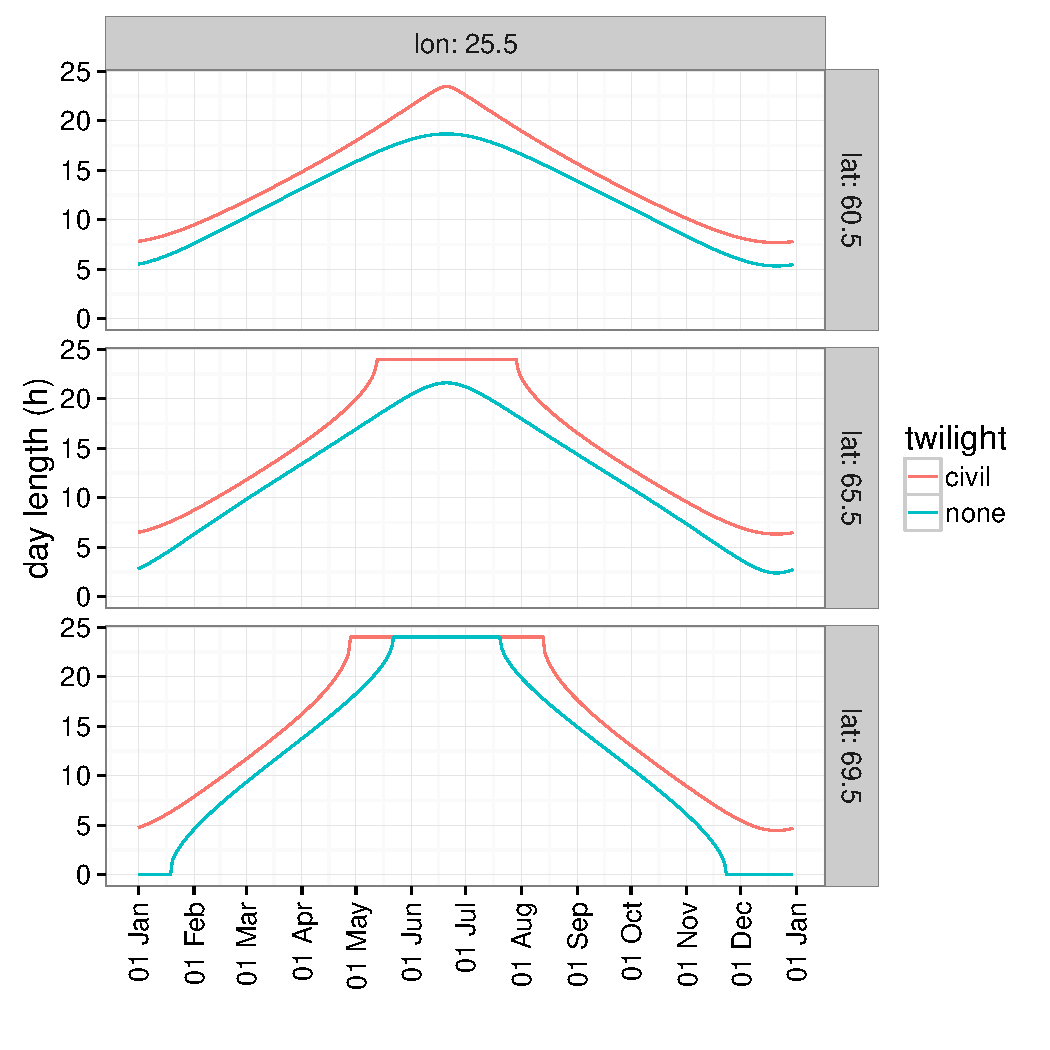
\includegraphics[width=0.6\linewidth]{figures/fig-anders4.pdf}
\end{frame}

\begin{frame}
  \frametitle{Temperature and its variability: 2004--2014}
  Large day to day variation at different latitudes (three grid points in Finland) = reliable only if averaged/accumulated.\\
  \centering
  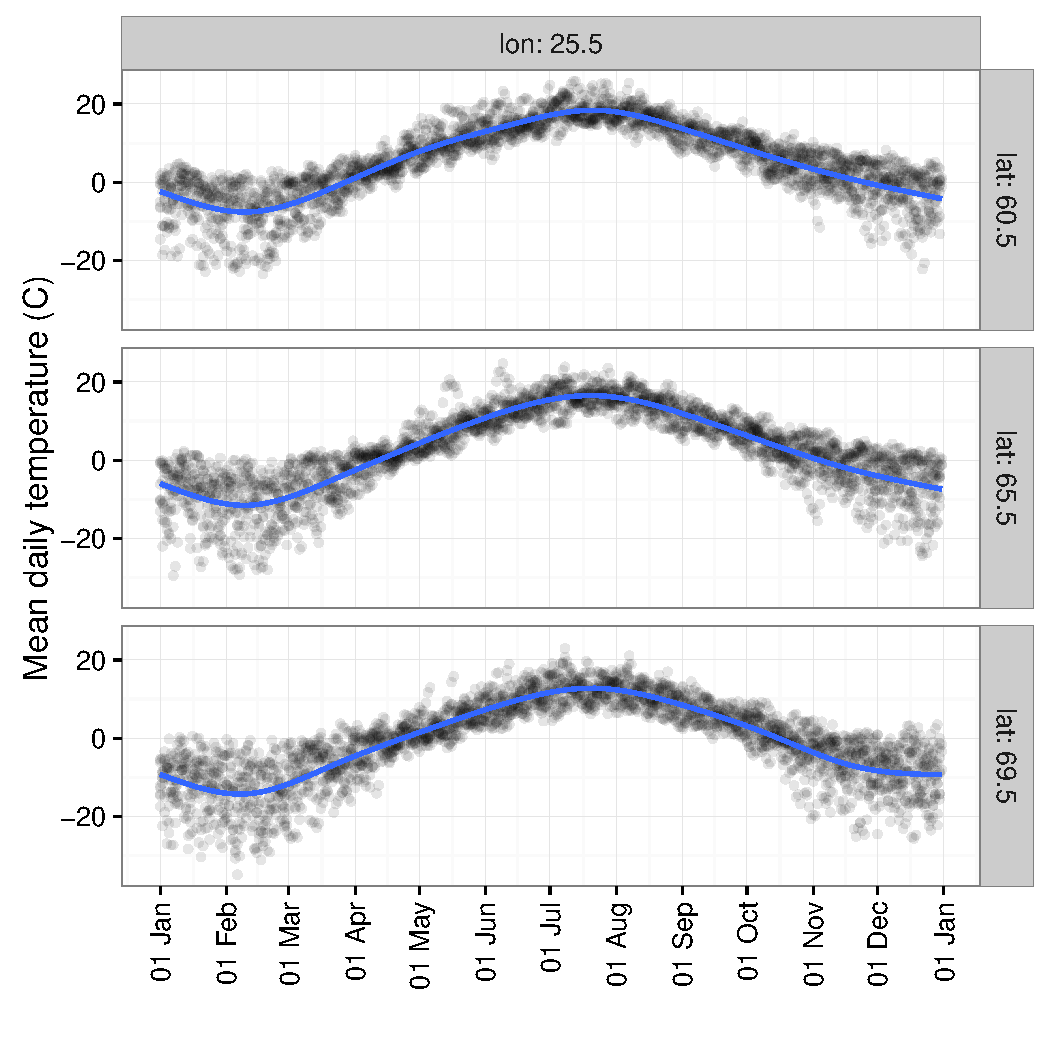
\includegraphics[width=0.6\linewidth]{figures/fig-anders2.pdf}

  (P. J. Aphalo, A. Lindfors, unpublished)
\end{frame}

%\begin{frame}
%  \frametitle{Global radiation and its variability: 2004--2014}
%  \centering
%  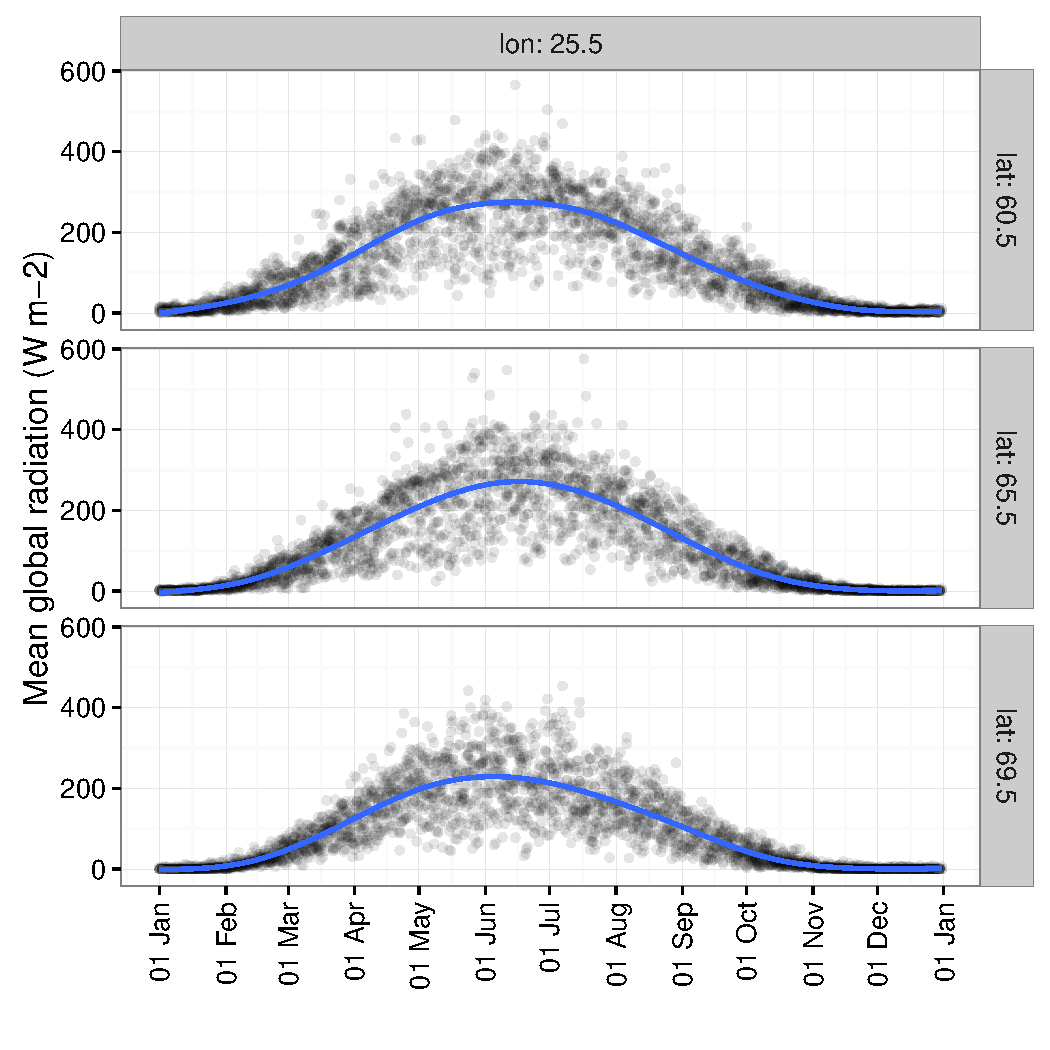
\includegraphics[width=0.65\linewidth]{figures/fig-anders3.pdf}
%
%  (P. J. Aphalo, A. Lindfors, unpublished)
%\end{frame}

\begin{frame}
  \frametitle{UV radiation and its variability: 2004--2014}
  \centering
  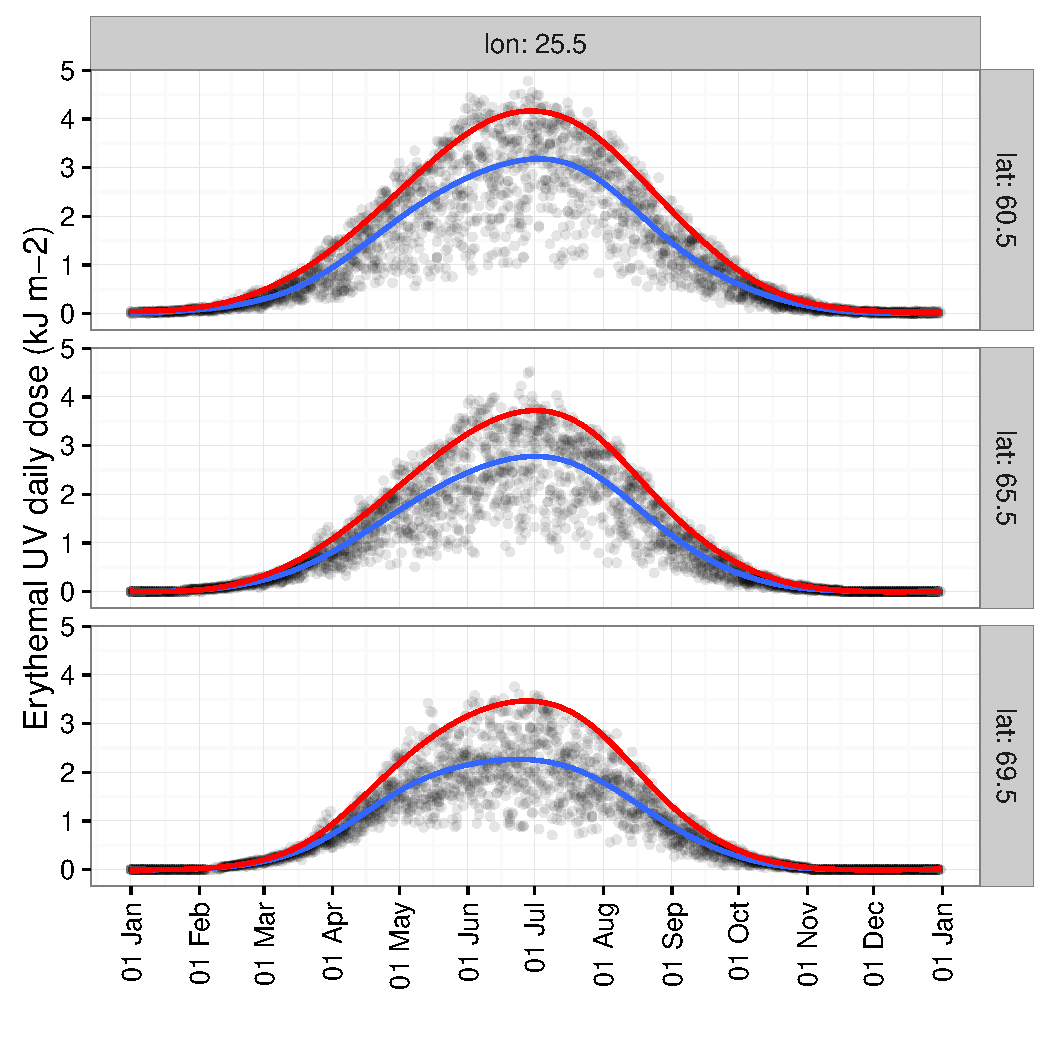
\includegraphics[width=0.65\linewidth]{figures/fig-anders1.pdf}

  (P. J. Aphalo, A. Lindfors, unpublished)
\end{frame}

\section[Preemptive acclimation to drought: available cues]{Preemptive acclimation to drought:\\ available cues}

\begin{frame}
  \frametitle{Soil water content as a cue}
   \begin{itemize}
    \item Plant roots can perceive dry soil (e.g.\ split root-system experiments) \ldots
    \item but, does this provide early-enough information for preemptive acclimation?
    \item Exposure to UV radiation can enhance drought tolerance\ldots
    \item Could exposure to UV radiation be an additional source of information?
  \end{itemize}
\end{frame}

\begin{frame}
  \frametitle{PET--UV correlation? Yes}
  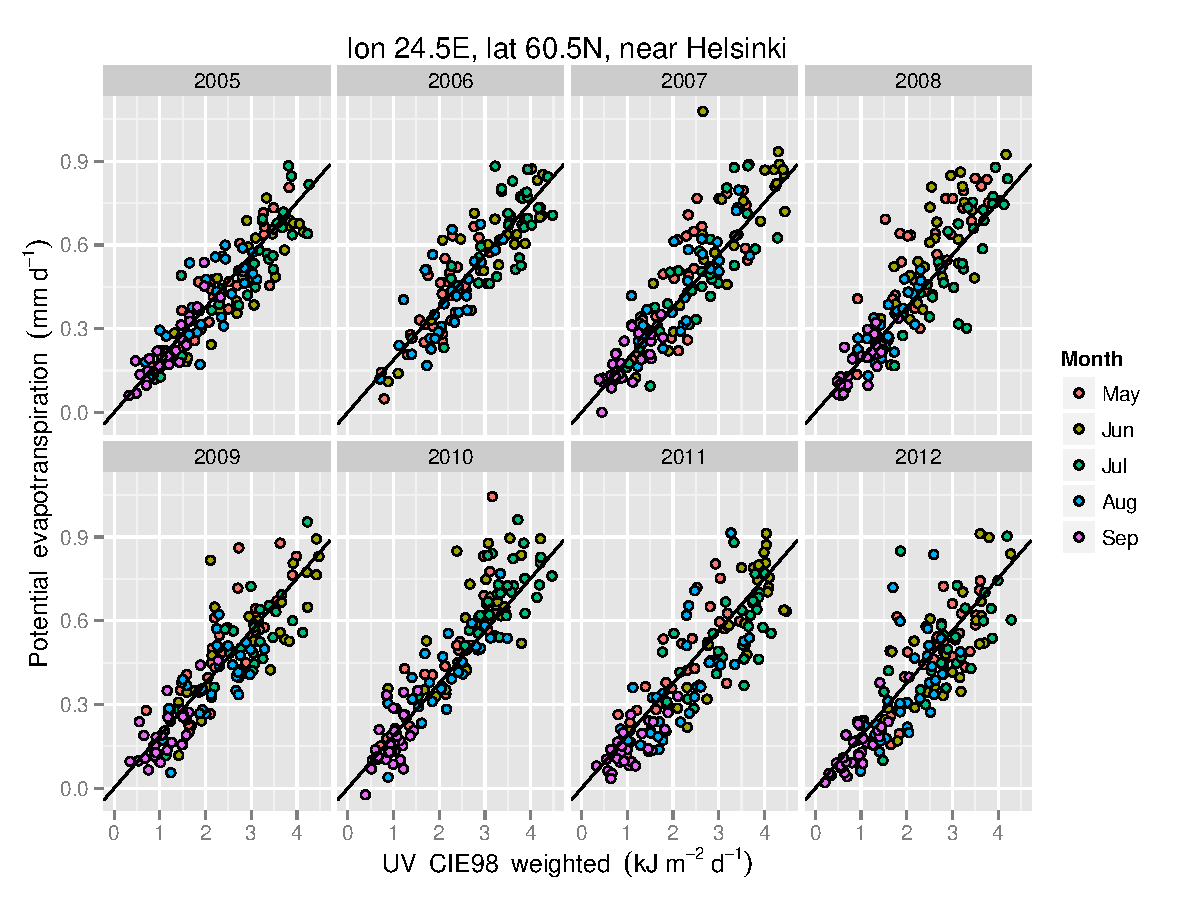
\includegraphics[width=0.8\linewidth]{figures/PET-CIE.pdf}

  (P. J. Aphalo, A. Lindfors, unpublished)
\end{frame}

\begin{frame}
  \frametitle{Soil water-UV correlation? Yes}
  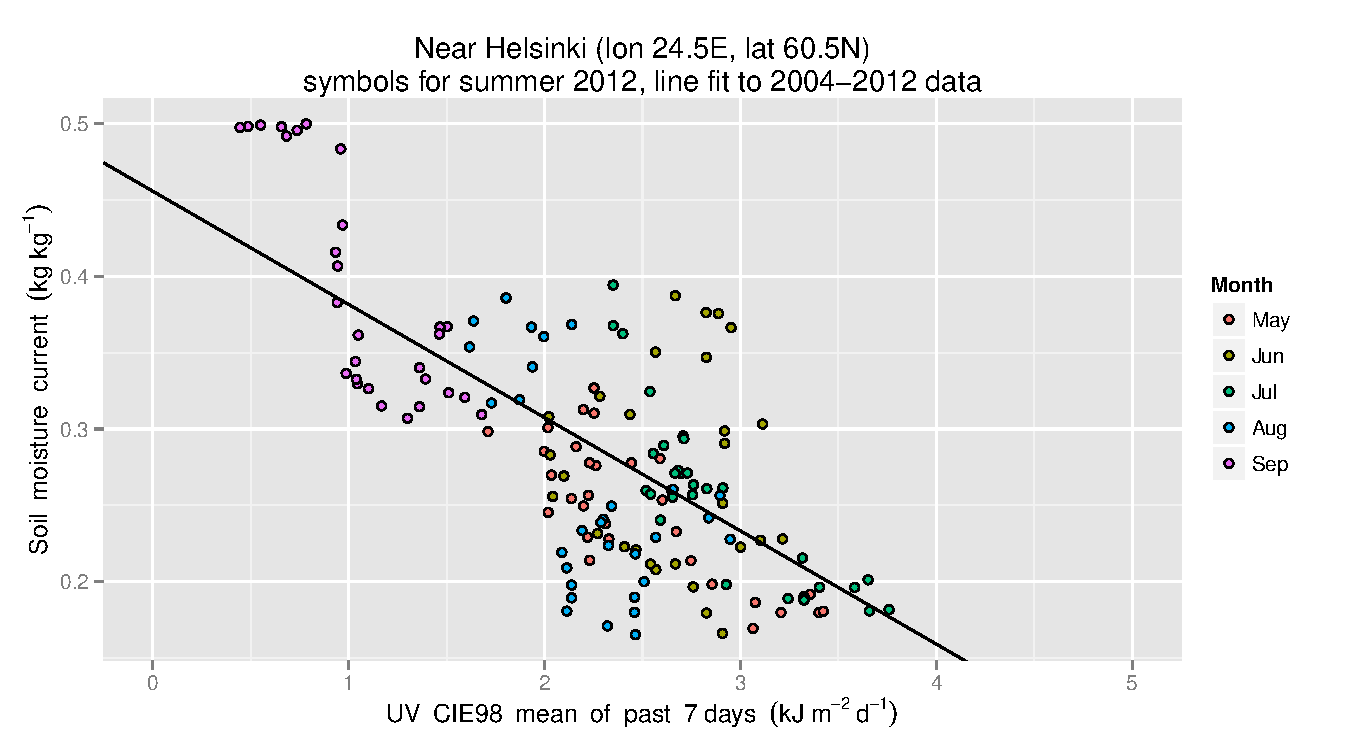
\includegraphics[width=\linewidth]{figures/soil-CIEmean.pdf}

  (P. J. Aphalo, A. Lindfors, unpublished)
\end{frame}

\section[Preemptive acclimation to drought: possible mechanism]{Preemptive acclimation to drought:\\ possible mechanism}

\begin{frame}
  \frametitle{Responses to growth under UV radiation}
   \begin{itemize}
    \item Smaller and thicker leaves
    \item Increased reflectance of leaves
    \item Slower opening of stomata when illuminated
    \item Compact growth habit
    \item Inhibition of shade avoidance responses driven by R:FR ratio
    \item Expression of genes related to ``water deprivation''\ldots
    \item \ldots aquaporins, proline synthesis, ABA signalling, stomatal responses to ABA
\end{itemize}
\end{frame}

\begin{frame}
  \frametitle{Signalling networks}
   \begin{itemize}
    \item Gene expression responses are interconnected and multiple interactions involved
    \item leading to very complex regulation.
    \item We can mostly get snapshots into a dynamic system
    \item The examples in the previous slide are convincing\ldots
    \item \ldots but cherry-picked from a long list
    \item Drought on the other hand triggers the expression of genes\ldots
    \item \ldots involved in light signalling
  \end{itemize}
\end{frame}

%\begin{frame}
%  \frametitle{Can exposure to UV-B trigger drought-acclimation? Yes}
%  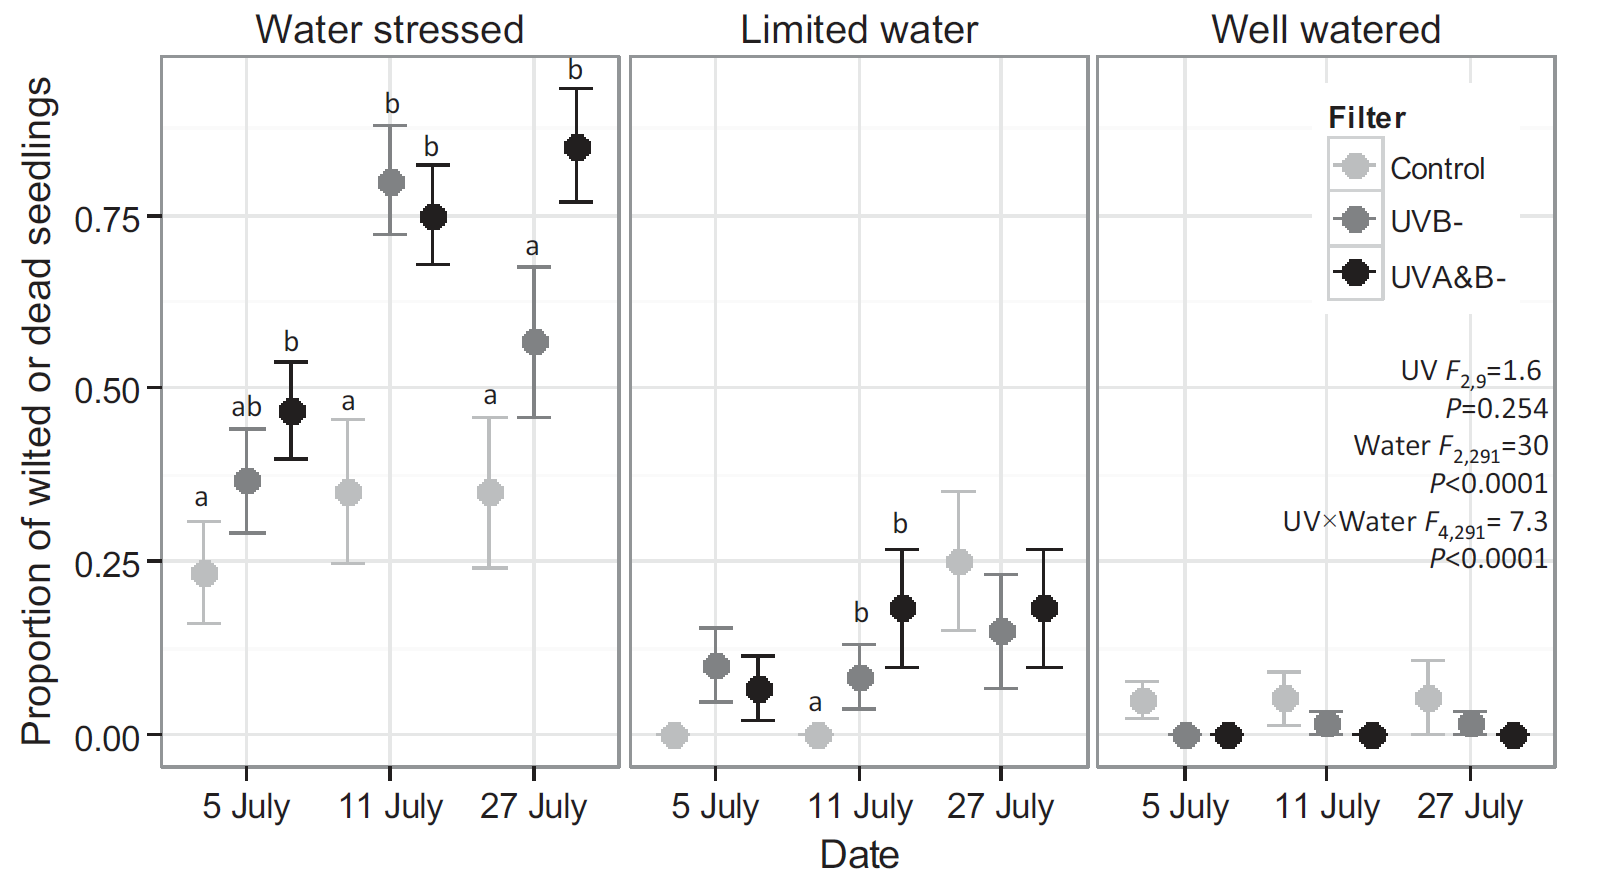
\includegraphics[width=\linewidth]{figures/birch-wilt.png}
%
%  \autocite{Robson2014}
%\end{frame}

%\begin{frame}
%  \frametitle{What about gene expression?}
%  From gene ontology (GO) terms enriched after UV-B exposure for 6~h.
%  \begin{itemize}
%    \item ``water transport'': genes including AT1G01620 (PIP1-3), AT2G37170 (PIP2B), AT3G16240 (TIP2-1), AT3G53420 (PIP2-1), AT3G61430 (PIP1-1), AT3G11820 (SYP121) and AT5G06530 (ABCG22).
%    \item ``response to water deprivation'': genes including AT1G20450 (ERD10), AT1G76180 (ERD14), AT2G30870 (ERD13), AT2G22430 (ATHB6), AT2G39800 (ATP5CS, proline synthesis), AT2G45960 (PIP1B), AT3G11410 (AHG3, ABA signalling), AT3G14050 (ATRSH2, ABA signalling), AT3G21780 (UGT71B6, ABA catabolism), AT5G57050 (ABI2, ABA, stomata).
%  \end{itemize}
%\end{frame}
%\begin{frame}[fragile]
%  \frametitle{Possible mechanisms: morphology? Yes or No}
%  <<biomass, echo = FALSE>>=
%biomass.df <- data.frame(shoot.biomass = c(0.2, 0.08, 0.17, 0.71, 0.56, 0.58, 1.36, 1.32, 1.35),
%                         shoot.biomass.sem = c(0.02, 0.01, 0.03, 0.02, 0.03, 0.03, 0.04, 0.05, 0.05),
%                         water.treatment = factor(rep(c("water stress", "water limited", "unrestricted"), c(3,3,3)),
%                                                  levels = c("water stress", "water limited", "unrestricted")),
%                         uv.treatment = factor(rep(c('full\nspectrum', "-UVB", "-UVB -UVA"), 3),
%                                               levels = c('full\nspectrum', "-UVB", "-UVB -UVA")))
%ggplot(biomass.df, aes(x = uv.treatment, y = shoot.biomass,
%                       ymin = shoot.biomass - shoot.biomass.sem,
%                       ymax = shoot.biomass + shoot.biomass.sem,
%                       colour = uv.treatment)) +
%geom_pointrange() +
%ylim(0, NA) +
%labs(x = "filter treatment", y = "Stem biomass (g)") +
%facet_wrap(~water.treatment)
%@
%\end{frame}
%
%%\begin{frame}
%%  \frametitle{Possible mechanisms: tissue water relations}
%%
%%\end{frame}
%
%\begin{frame}[fragile]
%  \frametitle{Possible mechanisms: stomatal conductance}
%<<echo=FALSE,fig.width=6, fig.height=4, out.width='.8\\textwidth'>>=
%load(file = "gs_light_summ.rda")
%ggplot(subset(gs_light_summ.df, blue != 0 & green == 0),
%         aes(treatment, gs_rate_mn * 60)) +
%  stat_summary(fun.data = "mean_se") + ylim(0, NA) +
%  labs(x = "Growth condition, filtered sunlight",
%       y = expression(Delta~g[s]/g[s]/Delta~t~~~("%"~min^{-1}))) +
%  ggtitle(expression(Opening~~speed~~of~~stomata~~"in"~~blue~~light~~~(italic(Tilia~~cordata))))
%@
%
%(K. Aasamaa and P. J. Aphalo, unpublished)
%\end{frame}

%\begin{frame}[fragile]
%  \frametitle{Possible mechanisms: stomatal conductance}
%<<echo=FALSE,fig.width=6, fig.height=4, out.width='.8\\textwidth'>>=
%load(file = "gs_light_summ.rda")
%ggplot(subset(gs_light_summ.df, blue != 0 & green == 0),
%         aes(treatment, gs_rate_mn * 60)) +
%  stat_summary(fun.data = "mean_se") + ylim(0, NA) +
%  labs(x = "Growth condition, filtered sunlight",
%       y = expression(Delta~g[s]/g[s]/Delta~t~~~("%"~min^{-1}))) +
%  ggtitle(expression(Opening~~speed~~of~~stomata~~"in"~~blue~~light~~~(italic(Tilia~~cordata))))
%@
%
%\autocite{Aasamaa2016}
%\end{frame}

%\begin{frame}
%  \frametitle{Possible mechanisms: gene expression}
%  \begin{itemize}
%    \item gene expression + Gene Ontology analysis
%       \begin{itemize}
%         \item Working on this (tried AgriGo, starting with Bioconductor topGO now)
%       \end{itemize}
%    \item gene expression + KEGG pathway analysis
%       \begin{itemize}
%         \item Bioconductor edgeR and topKEGG
%         \item Please see Neha Rai et al.'s poster.
%       \end{itemize}
%   \item Earlier observations on effects of UVB on genes related to
%      \begin{itemize}
%        \item phenolic metabolism
%        \item ABA signalling
%        \item energy metabolism
%        \item photosynthesis
%        \item cell growth
%      \end{itemize}
%  \end{itemize}
%\end{frame}

\section[Drought acclimation under UVB: possible implications]{Drought acclimation under UVB:\\ possible implications}

\begin{frame}
  \frametitle{Take home message from our research on UV}
  If our hypothesis holds for a range of species then there would be much to rethink:
  \begin{itemize}
    \item reduced growth under UV-B exposure could improve fitness instead of being deleterious,
    \item phenotyping for drought tolerance of dryland crops in the absence of UV-B could lead to suboptimal progress,
    \item what should we do with field crops under irrigation: do we need to breed out some of the UVB responses?,
    \item what about rain shelter experiments: should we supplement with UVB when it is cloudy or raining?
    \item What about climate change: should we acknowledge that changes in rainfall will correlate with changes in UVB due to cloud cover?
  \end{itemize}
\end{frame}

\begin{frame}
  \frametitle{Overall take home message}
  \begin{itemize}
    \item Exploring plants' growth environment as a source of information\ldots
    \item \ldots helps with the identification of ultimate causes\ldots
    \item \ldots and understanding these ultimate cuases\ldots
    \item \ldots could allow meaningful manipulation of proximate causes\ldots
    \item \ldots related to preemptive acclimation.
    \item Assuming that preemptive acclimation is crucial for plant adaptation and crop performance\ldots
    the need to consider the various contexts affecting crop breeding becomes obvious.
    \item e.g. ``taming'' of a partly preemptive response was behind the green revolution.
  \end{itemize}
\end{frame}

\begin{frame}
  \frametitle{A \emph{caveat}}
  \begin{itemize}
    \item The model I presented is mainly dealing, at least in my examples, with relatively ``normal business'', events that could take place every year to not more than a few generations apart.
    \item But boreal trees and plants have also survived as species very exceptional extreme events.
    \item This has also shaped the current genotypes, so do we need to also consider risk analysis when analysing the use of information by plants? and how?
  \end{itemize}
\end{frame}


%\begin{frame}[<+->]
%  \frametitle{Teaser: can you guess how long ago has this text been published?}
%\begin{quotation}
%\ldots the beneficial effects of ultraviolet
%on the animal organism have, in recent years, encouraged the
%attempt to demonstrate similar effects on plants, with the result that
%a great number of short experiments have been reported in which the
%lack of adequate controls has rendered the conclusions of doubtful
%value.
%
%\ldots\pause
%
%  The interest in
%ultra-violet in recent years has been so widespread as to justify the
%accusation of some that the subject is a fad. It is to be hoped that the
%"fad" will not run its course before accurate information has been
%obtained.
%\end{quotation}
%\pause
%\autocite{Popp1936}
%\end{frame}


\section{Acknowledgements}

\begin{frame}[t]
\begin{small}
\begin{tabular}{cp{0.7\textwidth}}
\href{http://blogs.helsinki.fi/senpep-blog/}{\pgfuseimage{SenPEP}} & \textbf{Members of my research group:} Sari Siipola, Fang Wang, Neha Rai, Yan Yan, Cyntia Ayala.\\
                                                                    & \textbf{Current collaborators:} Luis O. Morales, T. Matthew Robson, Anders Lindfors, \mbox{Víctor} Sadras, Jorge J. Casal, Saara Hartikainen, David Israel, Mikael Brosché, Tarja Lehto, Åke Strid, Gareth Jenkins, Andreas Albert, Fred Stoddard\\

\href{http://blogs.helsinki.fi/vips-blog/}{\pgfuseimage{ViPS}} & A new umbrella organization at our campus.\\

\href{http://www.helsinki.fi/en/}{\pgfuseimage{HYflame}} & My employer.\\

\href{http://www.aka.fi/en/}{\pgfuseimage{AKA}} & For funding, decisions 252548, 16775.\\

\end{tabular}
\end{small}

\end{frame}

\begin{frame}[allowframebreaks,t]
\printbibliography
\end{frame}

\begin{frame}%[<+->]
  \frametitle{Vocabulary: other terms}
  \begin{itemize}
    \item ``Plant neurobiology''.
    \item ``Plant intelligence''.
    \item In my view they are not useful.
    \item They are not abstract enough.
    \item They have an everyday meaning that is at odds with the proposed use.
    \item They distract us from the actual phenomena under study.
  \end{itemize}
\end{frame}

\begin{frame}
  \frametitle{Some connections to earlier talks}
  \begin{itemize}
    \item Veikko Koski's reference to ``Heisenberg's uncertainty principle'' triggered some thoughts: 1) the plants perceive the state of the environment but modify it, but also 2) in experiments we modify the environment, rather drastically, to study the responses of plants.
    \item In the discussion after Outi Savolainen's talk about the quantitative traits and the difficulties of dealing with many alleles the discussion centred on study methods. Later in the evening I started thinking whether having so many alleles could have a function in fitness. I came out with two ideas, at least the first one not original at all: 1) a smooth ``continuous'' range of possible daylength thresholds is good for fine tuning during ``normal business'', but 2) could this also be advantageous in ``extreme years'' as a way of preventing the loss of any alleles from the population even if a significant part of population with a non-hardy phenotype died.
  \end{itemize}
\end{frame}

\begin{frame}
  \frametitle{The origin of what I will present today}
  \begin{itemize}
    \item BSc Agronomy with emphasis in crop breeding (Genetics + Ecology + Statistics + Meteorology)
    \item MSc Plant Production (Ecophysiology + Sensory photobiology + Simulation modelling + General Systems Theory)
    \item - Computing programming + Systems analysis
    \item - Electronics + Instrumentation
    \item PhD in ``Science'' (Ecophysiology + Sensory photobiology + Instrumentation + Simulation modelling)
    \item METLA - seedling---seedling interactions + photobiology + growth regulators
    \item U. Joensuu - roots + cold + UVB radiation + Instrumentation + Computer Programming + Mineral Nutrition + Secondary metabolites
    \item U. Jyväskylä - statistics + time series analysis + UVB + Secondary metabolites
    \item U. Helsinki - add Heikki, molecular biology, a few additional plant species, a pinch of metabolomics and shake well
  \end{itemize}
\end{frame}

\end{document}

